\begin{frame}[fragile]{Visualização do algoritmo de Bellman-Ford}

    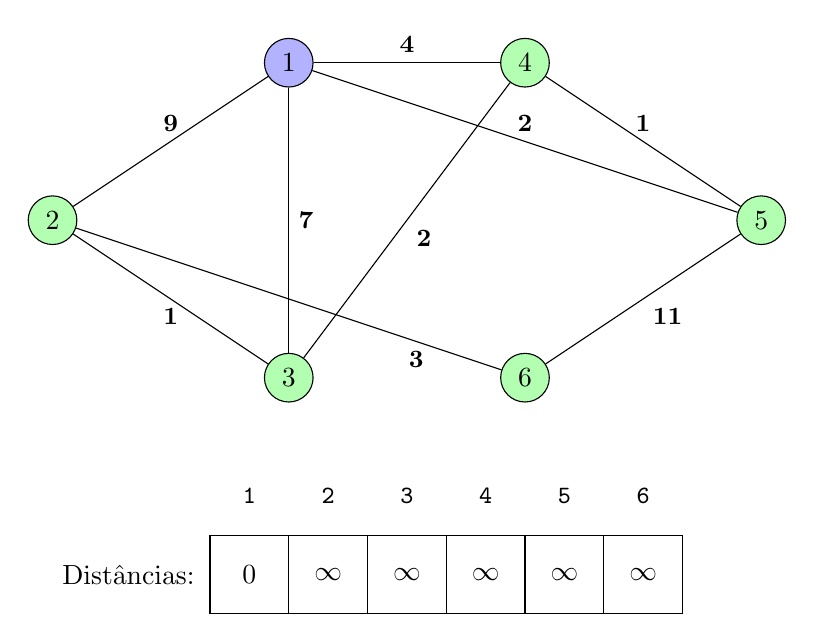
\begin{tikzpicture}
        \node[anchor=west] at (0, 0.5) { Distâncias: };

        \node[circle, draw, fill=blue!30] (a) at (3, 7) {1};
        \node[circle, draw, fill=green!30] (b) at (0, 5) {2};
        \node[circle, draw, fill=green!30] (c) at (3, 3) {3};
        \node[circle, draw, fill=green!30] (d) at (6, 7) {4};
        \node[circle, draw, fill=green!30] (e) at (9, 5) {5};
        \node[circle, draw, fill=green!30] (f) at (6, 3) {6};

        \draw (2, 0) grid (8, 1);

        \node at (2.5, 0.5) { $0$ };
        \node at (3.5, 0.5) { $\infty$ };
        \node at (4.5, 0.5) { $\infty$ };
        \node at (5.5, 0.5) { $\infty$ };
        \node at (6.5, 0.5) { $\infty$ };
        \node at (7.5, 0.5) { $\infty$ };

        \node at (2.5, 1.5) { \small \texttt{1} };
        \node at (3.5, 1.5) { \small \texttt{2} };
        \node at (4.5, 1.5) { \small \texttt{3} };
        \node at (5.5, 1.5) { \small \texttt{4} };
        \node at (6.5, 1.5) { \small \texttt{5} };
        \node at (7.5, 1.5) { \small \texttt{6} };

        \draw (a) to node[midway,anchor=south] { \small \bfseries 9 } (b);
        \draw (a) to node[midway,anchor=west] { \small \bfseries 7 } (c);
        \draw (a) to node[midway,anchor=south] { \small \bfseries 4 } (d);
        \draw (a) to node[midway,anchor=south] { \small \bfseries 2 } (e);
        \draw (b) to node[midway,anchor=north] { \small \bfseries 1 } (c);
        \draw (b) to node[pos=0.8,anchor=north] { \small \bfseries 3 } (f);
        \draw (c) to node[midway,anchor=north west] { \small \bfseries 2 } (d);
        \draw (d) to node[midway,anchor=south] { \small \bfseries 1 } (e);
        \draw (e) to node[midway,anchor=north west] { \small \bfseries 11 } (f);

    \end{tikzpicture}

\end{frame}

\begin{frame}[fragile]{Visualização do algoritmo de Bellman-Ford}

    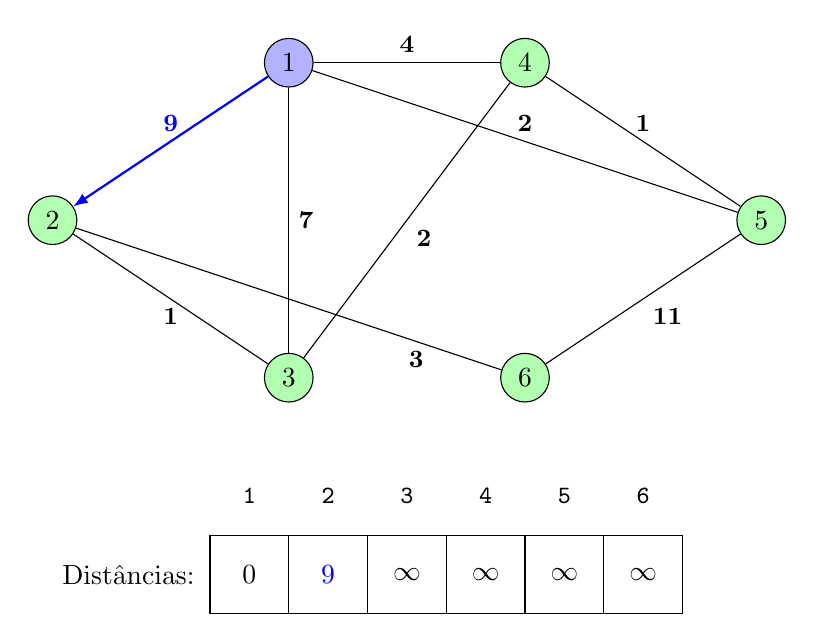
\begin{tikzpicture}
        \node[anchor=west] at (0, 0.5) { Distâncias: };

        \node[circle, draw, fill=blue!30] (a) at (3, 7) {1};
        \node[circle, draw, fill=green!30] (b) at (0, 5) {2};
        \node[circle, draw, fill=green!30] (c) at (3, 3) {3};
        \node[circle, draw, fill=green!30] (d) at (6, 7) {4};
        \node[circle, draw, fill=green!30] (e) at (9, 5) {5};
        \node[circle, draw, fill=green!30] (f) at (6, 3) {6};

        \draw (2, 0) grid (8, 1);

        \node at (2.5, 0.5) { $0$ };
        \node at (3.5, 0.5) { \textcolor{blue}{$9$} };
        \node at (4.5, 0.5) { $\infty$ };
        \node at (5.5, 0.5) { $\infty$ };
        \node at (6.5, 0.5) { $\infty$ };
        \node at (7.5, 0.5) { $\infty$ };

        \node at (2.5, 1.5) { \small \texttt{1} };
        \node at (3.5, 1.5) { \small \texttt{2} };
        \node at (4.5, 1.5) { \small \texttt{3} };
        \node at (5.5, 1.5) { \small \texttt{4} };
        \node at (6.5, 1.5) { \small \texttt{5} };
        \node at (7.5, 1.5) { \small \texttt{6} };

        \draw[-latex,thick,blue] (a) to node[midway,anchor=south] { \small \bfseries 9 } (b);
        %\draw (a) to node[midway,anchor=south] { \small \bfseries 9 } (b);
        \draw (a) to node[midway,anchor=west] { \small \bfseries 7 } (c);
        \draw (a) to node[midway,anchor=south] { \small \bfseries 4 } (d);
        \draw (a) to node[midway,anchor=south] { \small \bfseries 2 } (e);
        \draw (b) to node[midway,anchor=north] { \small \bfseries 1 } (c);
        \draw (b) to node[pos=0.8,anchor=north] { \small \bfseries 3 } (f);
        \draw (c) to node[midway,anchor=north west] { \small \bfseries 2 } (d);
        \draw (d) to node[midway,anchor=south] { \small \bfseries 1 } (e);
        \draw (e) to node[midway,anchor=north west] { \small \bfseries 11 } (f);

    \end{tikzpicture}

\end{frame}

\begin{frame}[fragile]{Visualização do algoritmo de Bellman-Ford}

    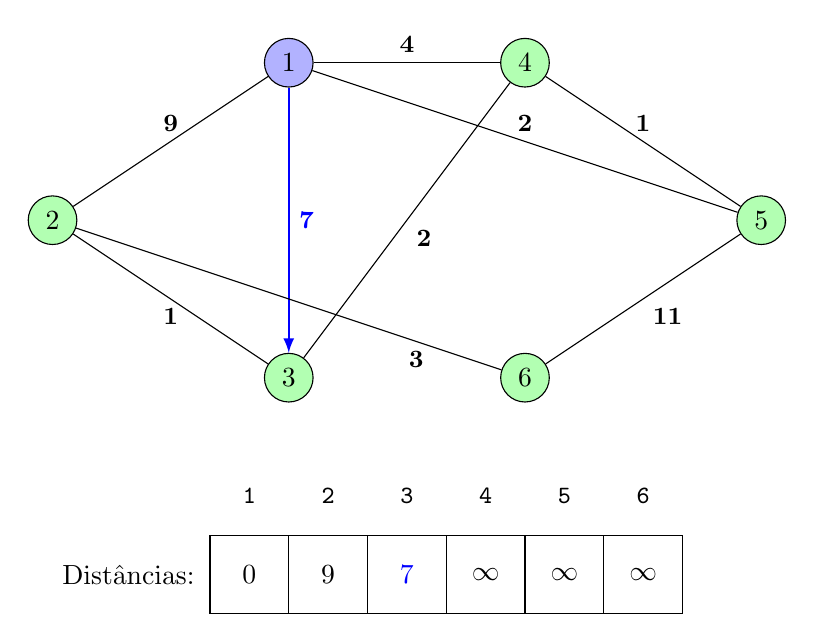
\begin{tikzpicture}
        \node[anchor=west] at (0, 0.5) { Distâncias: };

        \node[circle, draw, fill=blue!30] (a) at (3, 7) {1};
        \node[circle, draw, fill=green!30] (b) at (0, 5) {2};
        \node[circle, draw, fill=green!30] (c) at (3, 3) {3};
        \node[circle, draw, fill=green!30] (d) at (6, 7) {4};
        \node[circle, draw, fill=green!30] (e) at (9, 5) {5};
        \node[circle, draw, fill=green!30] (f) at (6, 3) {6};

        \draw (2, 0) grid (8, 1);

        \node at (2.5, 0.5) { $0$ };
        \node at (3.5, 0.5) { \textcolor{black}{$9$} };
        \node at (4.5, 0.5) { \textcolor{blue}{$7$} };
        \node at (5.5, 0.5) { $\infty$ };
        \node at (6.5, 0.5) { $\infty$ };
        \node at (7.5, 0.5) { $\infty$ };

        \node at (2.5, 1.5) { \small \texttt{1} };
        \node at (3.5, 1.5) { \small \texttt{2} };
        \node at (4.5, 1.5) { \small \texttt{3} };
        \node at (5.5, 1.5) { \small \texttt{4} };
        \node at (6.5, 1.5) { \small \texttt{5} };
        \node at (7.5, 1.5) { \small \texttt{6} };

        \draw (a) to node[midway,anchor=south] { \small \bfseries 9 } (b);
        %\draw (a) to node[midway,anchor=west] { \small \bfseries 7 } (c);
        \draw[-latex,thick,blue] (a) to node[midway,anchor=west] { \small \bfseries 7 } (c);
        \draw (a) to node[midway,anchor=south] { \small \bfseries 4 } (d);
        \draw (a) to node[midway,anchor=south] { \small \bfseries 2 } (e);
        \draw (b) to node[midway,anchor=north] { \small \bfseries 1 } (c);
        \draw (b) to node[pos=0.8,anchor=north] { \small \bfseries 3 } (f);
        \draw (c) to node[midway,anchor=north west] { \small \bfseries 2 } (d);
        \draw (d) to node[midway,anchor=south] { \small \bfseries 1 } (e);
        \draw (e) to node[midway,anchor=north west] { \small \bfseries 11 } (f);

    \end{tikzpicture}

\end{frame}

\begin{frame}[fragile]{Visualização do algoritmo de Bellman-Ford}

    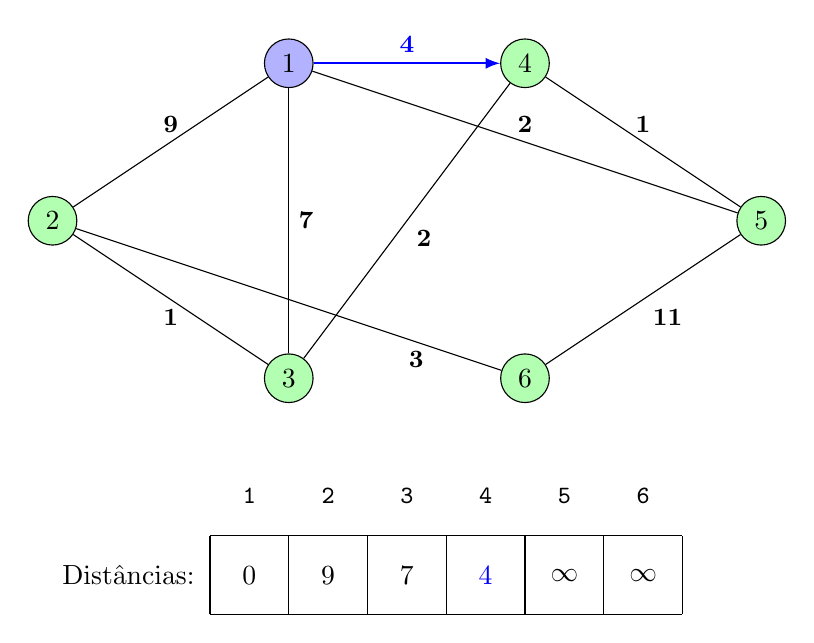
\begin{tikzpicture}
        \node[anchor=west] at (0, 0.5) { Distâncias: };

        \node[circle, draw, fill=blue!30] (a) at (3, 7) {1};
        \node[circle, draw, fill=green!30] (b) at (0, 5) {2};
        \node[circle, draw, fill=green!30] (c) at (3, 3) {3};
        \node[circle, draw, fill=green!30] (d) at (6, 7) {4};
        \node[circle, draw, fill=green!30] (e) at (9, 5) {5};
        \node[circle, draw, fill=green!30] (f) at (6, 3) {6};

        \draw (2, 0) grid (8, 1);

        \node at (2.5, 0.5) { $0$ };
        \node at (3.5, 0.5) { \textcolor{black}{$9$} };
        \node at (4.5, 0.5) { \textcolor{black}{$7$} };
        \node at (5.5, 0.5) { \textcolor{blue}{$4$} };
        \node at (6.5, 0.5) { $\infty$ };
        \node at (7.5, 0.5) { $\infty$ };

        \node at (2.5, 1.5) { \small \texttt{1} };
        \node at (3.5, 1.5) { \small \texttt{2} };
        \node at (4.5, 1.5) { \small \texttt{3} };
        \node at (5.5, 1.5) { \small \texttt{4} };
        \node at (6.5, 1.5) { \small \texttt{5} };
        \node at (7.5, 1.5) { \small \texttt{6} };

        \draw (a) to node[midway,anchor=south] { \small \bfseries 9 } (b);
        \draw (a) to node[midway,anchor=west] { \small \bfseries 7 } (c);
        %\draw (a) to node[midway,anchor=south] { \small \bfseries 4 } (d);
        \draw[-latex,thick,blue] (a) to node[midway,anchor=south] { \small \bfseries 4 } (d);
        \draw (a) to node[midway,anchor=south] { \small \bfseries 2 } (e);
        \draw (b) to node[midway,anchor=north] { \small \bfseries 1 } (c);
        \draw (b) to node[pos=0.8,anchor=north] { \small \bfseries 3 } (f);
        \draw (c) to node[midway,anchor=north west] { \small \bfseries 2 } (d);
        \draw (d) to node[midway,anchor=south] { \small \bfseries 1 } (e);
        \draw (e) to node[midway,anchor=north west] { \small \bfseries 11 } (f);

    \end{tikzpicture}

\end{frame}

\begin{frame}[fragile]{Visualização do algoritmo de Bellman-Ford}

    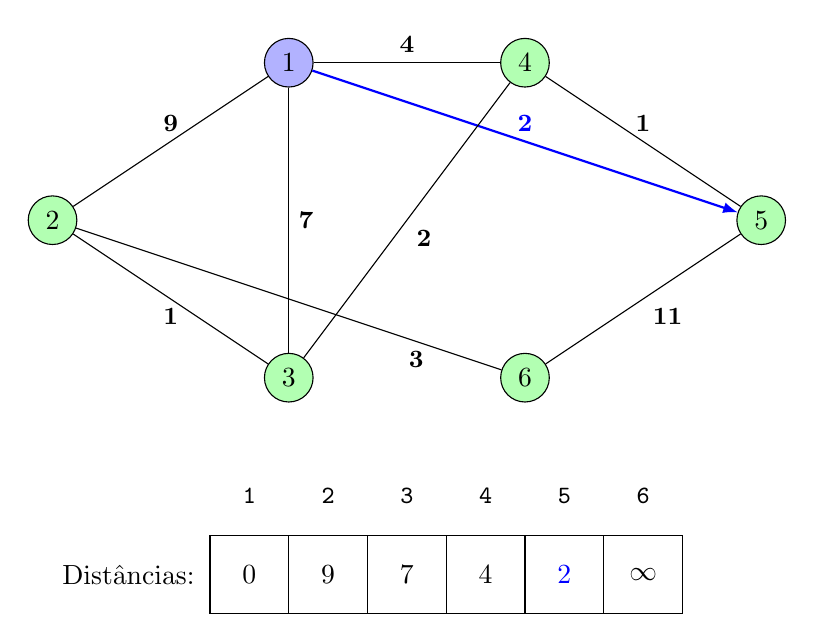
\begin{tikzpicture}
        \node[anchor=west] at (0, 0.5) { Distâncias: };

        \node[circle, draw, fill=blue!30] (a) at (3, 7) {1};
        \node[circle, draw, fill=green!30] (b) at (0, 5) {2};
        \node[circle, draw, fill=green!30] (c) at (3, 3) {3};
        \node[circle, draw, fill=green!30] (d) at (6, 7) {4};
        \node[circle, draw, fill=green!30] (e) at (9, 5) {5};
        \node[circle, draw, fill=green!30] (f) at (6, 3) {6};

        \draw (2, 0) grid (8, 1);

        \node at (2.5, 0.5) { $0$ };
        \node at (3.5, 0.5) { \textcolor{black}{$9$} };
        \node at (4.5, 0.5) { \textcolor{black}{$7$} };
        \node at (5.5, 0.5) { \textcolor{black}{$4$} };
        \node at (6.5, 0.5) { \textcolor{blue}{$2$} };
        \node at (7.5, 0.5) { $\infty$ };

        \node at (2.5, 1.5) { \small \texttt{1} };
        \node at (3.5, 1.5) { \small \texttt{2} };
        \node at (4.5, 1.5) { \small \texttt{3} };
        \node at (5.5, 1.5) { \small \texttt{4} };
        \node at (6.5, 1.5) { \small \texttt{5} };
        \node at (7.5, 1.5) { \small \texttt{6} };

        \draw (a) to node[midway,anchor=south] { \small \bfseries 9 } (b);
        \draw (a) to node[midway,anchor=west] { \small \bfseries 7 } (c);
        \draw (a) to node[midway,anchor=south] { \small \bfseries 4 } (d);
        %\draw (a) to node[midway,anchor=south] { \small \bfseries 2 } (e);
        \draw[-latex,thick,blue] (a) to node[midway,anchor=south] { \small \bfseries 2 } (e);
        \draw (b) to node[midway,anchor=north] { \small \bfseries 1 } (c);
        \draw (b) to node[pos=0.8,anchor=north] { \small \bfseries 3 } (f);
        \draw (c) to node[midway,anchor=north west] { \small \bfseries 2 } (d);
        \draw (d) to node[midway,anchor=south] { \small \bfseries 1 } (e);
        \draw (e) to node[midway,anchor=north west] { \small \bfseries 11 } (f);

    \end{tikzpicture}

\end{frame}

\begin{frame}[fragile]{Visualização do algoritmo de Bellman-Ford}

    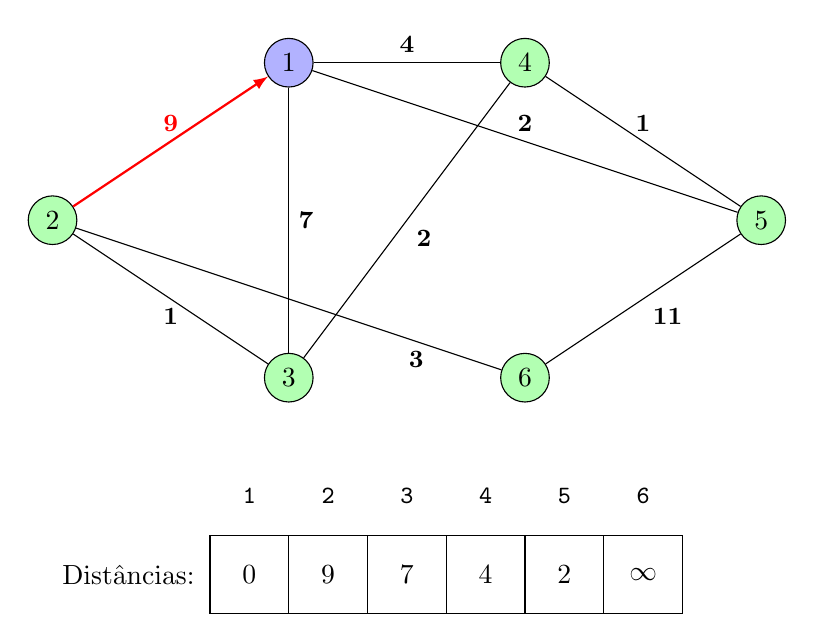
\begin{tikzpicture}
        \node[anchor=west] at (0, 0.5) { Distâncias: };

        \node[circle, draw, fill=blue!30] (a) at (3, 7) {1};
        \node[circle, draw, fill=green!30] (b) at (0, 5) {2};
        \node[circle, draw, fill=green!30] (c) at (3, 3) {3};
        \node[circle, draw, fill=green!30] (d) at (6, 7) {4};
        \node[circle, draw, fill=green!30] (e) at (9, 5) {5};
        \node[circle, draw, fill=green!30] (f) at (6, 3) {6};

        \draw (2, 0) grid (8, 1);

        \node at (2.5, 0.5) { $0$ };
        \node at (3.5, 0.5) { \textcolor{black}{$9$} };
        \node at (4.5, 0.5) { \textcolor{black}{$7$} };
        \node at (5.5, 0.5) { \textcolor{black}{$4$} };
        \node at (6.5, 0.5) { \textcolor{black}{$2$} };
        \node at (7.5, 0.5) { $\infty$ };

        \node at (2.5, 1.5) { \small \texttt{1} };
        \node at (3.5, 1.5) { \small \texttt{2} };
        \node at (4.5, 1.5) { \small \texttt{3} };
        \node at (5.5, 1.5) { \small \texttt{4} };
        \node at (6.5, 1.5) { \small \texttt{5} };
        \node at (7.5, 1.5) { \small \texttt{6} };

        \draw[latex-,thick,red] (a) to node[midway,anchor=south] { \small \bfseries 9 } (b);
        \draw (a) to node[midway,anchor=west] { \small \bfseries 7 } (c);
        \draw (a) to node[midway,anchor=south] { \small \bfseries 4 } (d);
        \draw (a) to node[midway,anchor=south] { \small \bfseries 2 } (e);
        \draw (b) to node[midway,anchor=north] { \small \bfseries 1 } (c);
        \draw (b) to node[pos=0.8,anchor=north] { \small \bfseries 3 } (f);
        \draw (c) to node[midway,anchor=north west] { \small \bfseries 2 } (d);
        \draw (d) to node[midway,anchor=south] { \small \bfseries 1 } (e);
        \draw (e) to node[midway,anchor=north west] { \small \bfseries 11 } (f);

    \end{tikzpicture}

\end{frame}

\begin{frame}[fragile]{Visualização do algoritmo de Bellman-Ford}

    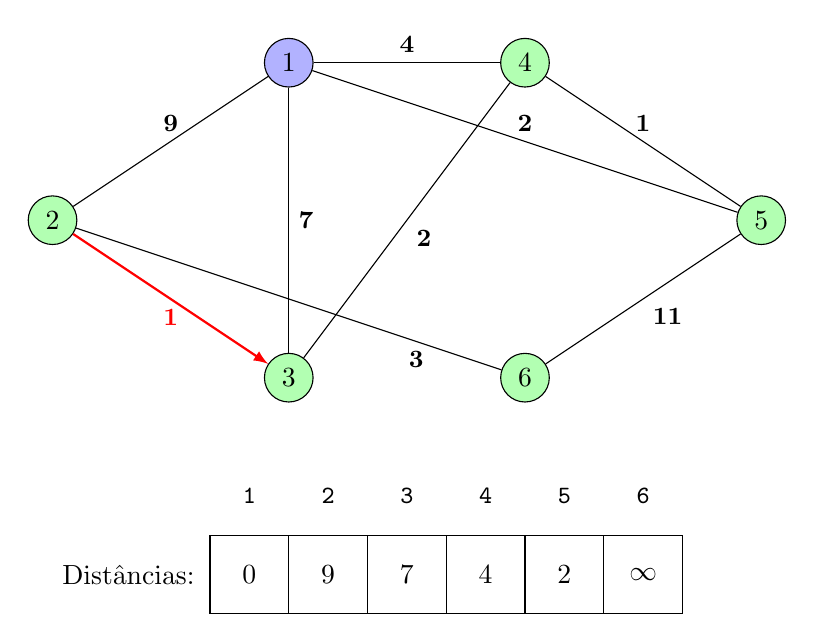
\begin{tikzpicture}
        \node[anchor=west] at (0, 0.5) { Distâncias: };

        \node[circle, draw, fill=blue!30] (a) at (3, 7) {1};
        \node[circle, draw, fill=green!30] (b) at (0, 5) {2};
        \node[circle, draw, fill=green!30] (c) at (3, 3) {3};
        \node[circle, draw, fill=green!30] (d) at (6, 7) {4};
        \node[circle, draw, fill=green!30] (e) at (9, 5) {5};
        \node[circle, draw, fill=green!30] (f) at (6, 3) {6};

        \draw (2, 0) grid (8, 1);

        \node at (2.5, 0.5) { $0$ };
        \node at (3.5, 0.5) { \textcolor{black}{$9$} };
        \node at (4.5, 0.5) { \textcolor{black}{$7$} };
        \node at (5.5, 0.5) { \textcolor{black}{$4$} };
        \node at (6.5, 0.5) { \textcolor{black}{$2$} };
        \node at (7.5, 0.5) { $\infty$ };

        \node at (2.5, 1.5) { \small \texttt{1} };
        \node at (3.5, 1.5) { \small \texttt{2} };
        \node at (4.5, 1.5) { \small \texttt{3} };
        \node at (5.5, 1.5) { \small \texttt{4} };
        \node at (6.5, 1.5) { \small \texttt{5} };
        \node at (7.5, 1.5) { \small \texttt{6} };

        \draw (a) to node[midway,anchor=south] { \small \bfseries 9 } (b);
        \draw (a) to node[midway,anchor=west] { \small \bfseries 7 } (c);
        \draw (a) to node[midway,anchor=south] { \small \bfseries 4 } (d);
        \draw (a) to node[midway,anchor=south] { \small \bfseries 2 } (e);
        %\draw (b) to node[midway,anchor=north] { \small \bfseries 1 } (c);
        \draw[-latex,thick,red] (b) to node[midway,anchor=north] { \small \bfseries 1 } (c);
        \draw (b) to node[pos=0.8,anchor=north] { \small \bfseries 3 } (f);
        \draw (c) to node[midway,anchor=north west] { \small \bfseries 2 } (d);
        \draw (d) to node[midway,anchor=south] { \small \bfseries 1 } (e);
        \draw (e) to node[midway,anchor=north west] { \small \bfseries 11 } (f);

    \end{tikzpicture}

\end{frame}

\begin{frame}[fragile]{Visualização do algoritmo de Bellman-Ford}

    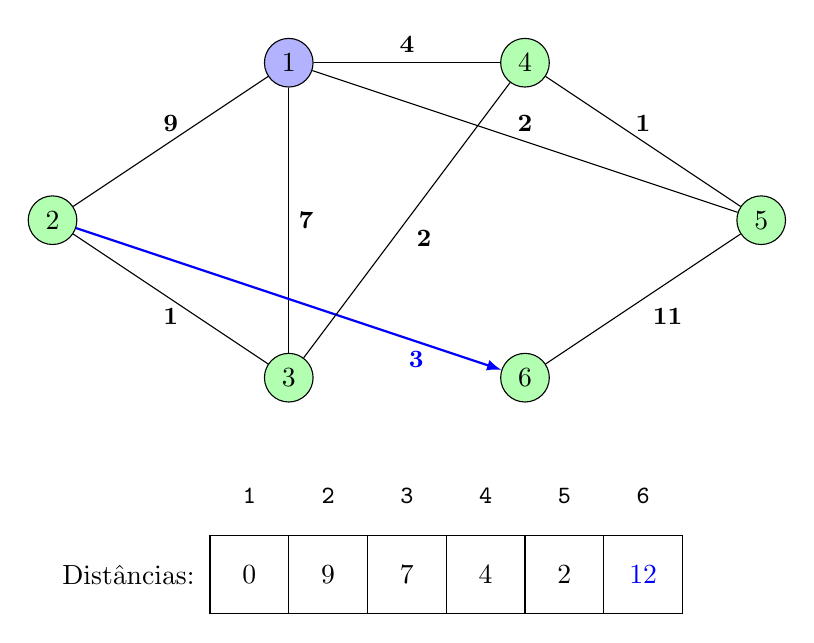
\begin{tikzpicture}
        \node[anchor=west] at (0, 0.5) { Distâncias: };

        \node[circle, draw, fill=blue!30] (a) at (3, 7) {1};
        \node[circle, draw, fill=green!30] (b) at (0, 5) {2};
        \node[circle, draw, fill=green!30] (c) at (3, 3) {3};
        \node[circle, draw, fill=green!30] (d) at (6, 7) {4};
        \node[circle, draw, fill=green!30] (e) at (9, 5) {5};
        \node[circle, draw, fill=green!30] (f) at (6, 3) {6};

        \draw (2, 0) grid (8, 1);

        \node at (2.5, 0.5) { $0$ };
        \node at (3.5, 0.5) { \textcolor{black}{$9$} };
        \node at (4.5, 0.5) { \textcolor{black}{$7$} };
        \node at (5.5, 0.5) { \textcolor{black}{$4$} };
        \node at (6.5, 0.5) { \textcolor{black}{$2$} };
        \node at (7.5, 0.5) { \textcolor{blue}{$12$} };

        \node at (2.5, 1.5) { \small \texttt{1} };
        \node at (3.5, 1.5) { \small \texttt{2} };
        \node at (4.5, 1.5) { \small \texttt{3} };
        \node at (5.5, 1.5) { \small \texttt{4} };
        \node at (6.5, 1.5) { \small \texttt{5} };
        \node at (7.5, 1.5) { \small \texttt{6} };

        \draw (a) to node[midway,anchor=south] { \small \bfseries 9 } (b);
        \draw (a) to node[midway,anchor=west] { \small \bfseries 7 } (c);
        \draw (a) to node[midway,anchor=south] { \small \bfseries 4 } (d);
        \draw (a) to node[midway,anchor=south] { \small \bfseries 2 } (e);
        \draw (b) to node[midway,anchor=north] { \small \bfseries 1 } (c);
        %\draw (b) to node[pos=0.8,anchor=north] { \small \bfseries 3 } (f);
        \draw[-latex,thick,blue] (b) to node[pos=0.8,anchor=north] { \small \bfseries 3 } (f);
        \draw (c) to node[midway,anchor=north west] { \small \bfseries 2 } (d);
        \draw (d) to node[midway,anchor=south] { \small \bfseries 1 } (e);
        \draw (e) to node[midway,anchor=north west] { \small \bfseries 11 } (f);

    \end{tikzpicture}

\end{frame}

\begin{frame}[fragile]{Visualização do algoritmo de Bellman-Ford}

    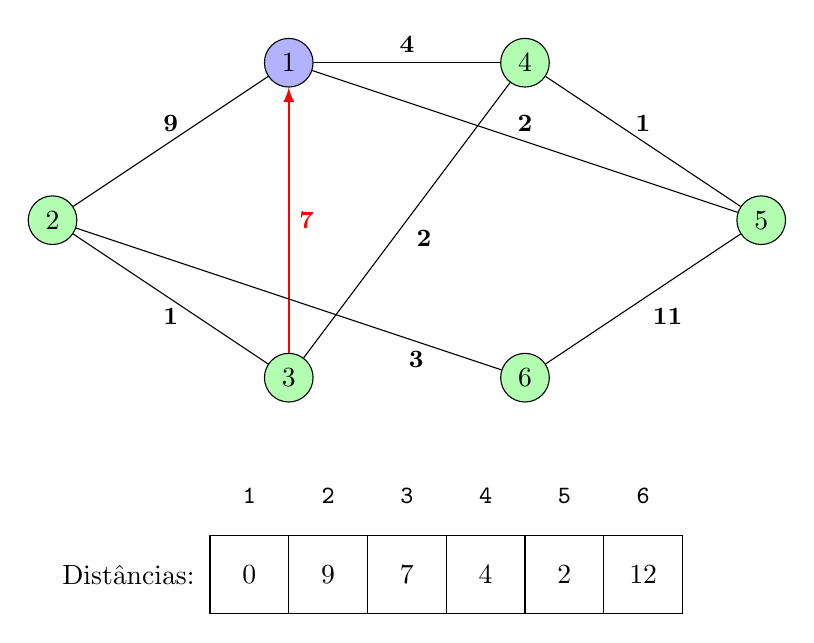
\begin{tikzpicture}
        \node[anchor=west] at (0, 0.5) { Distâncias: };

        \node[circle, draw, fill=blue!30] (a) at (3, 7) {1};
        \node[circle, draw, fill=green!30] (b) at (0, 5) {2};
        \node[circle, draw, fill=green!30] (c) at (3, 3) {3};
        \node[circle, draw, fill=green!30] (d) at (6, 7) {4};
        \node[circle, draw, fill=green!30] (e) at (9, 5) {5};
        \node[circle, draw, fill=green!30] (f) at (6, 3) {6};

        \draw (2, 0) grid (8, 1);

        \node at (2.5, 0.5) { $0$ };
        \node at (3.5, 0.5) { \textcolor{black}{$9$} };
        \node at (4.5, 0.5) { \textcolor{black}{$7$} };
        \node at (5.5, 0.5) { \textcolor{black}{$4$} };
        \node at (6.5, 0.5) { \textcolor{black}{$2$} };
        \node at (7.5, 0.5) { \textcolor{black}{$12$} };

        \node at (2.5, 1.5) { \small \texttt{1} };
        \node at (3.5, 1.5) { \small \texttt{2} };
        \node at (4.5, 1.5) { \small \texttt{3} };
        \node at (5.5, 1.5) { \small \texttt{4} };
        \node at (6.5, 1.5) { \small \texttt{5} };
        \node at (7.5, 1.5) { \small \texttt{6} };

        \draw (a) to node[midway,anchor=south] { \small \bfseries 9 } (b);
        %\draw (a) to node[midway,anchor=west] { \small \bfseries 7 } (c);
        \draw[latex-,thick,red] (a) to node[midway,anchor=west] { \small \bfseries 7 } (c);
        \draw (a) to node[midway,anchor=south] { \small \bfseries 4 } (d);
        \draw (a) to node[midway,anchor=south] { \small \bfseries 2 } (e);
        \draw (b) to node[midway,anchor=north] { \small \bfseries 1 } (c);
        \draw (b) to node[pos=0.8,anchor=north] { \small \bfseries 3 } (f);
        \draw (c) to node[midway,anchor=north west] { \small \bfseries 2 } (d);
        \draw (d) to node[midway,anchor=south] { \small \bfseries 1 } (e);
        \draw (e) to node[midway,anchor=north west] { \small \bfseries 11 } (f);

    \end{tikzpicture}

\end{frame}

\begin{frame}[fragile]{Visualização do algoritmo de Bellman-Ford}

    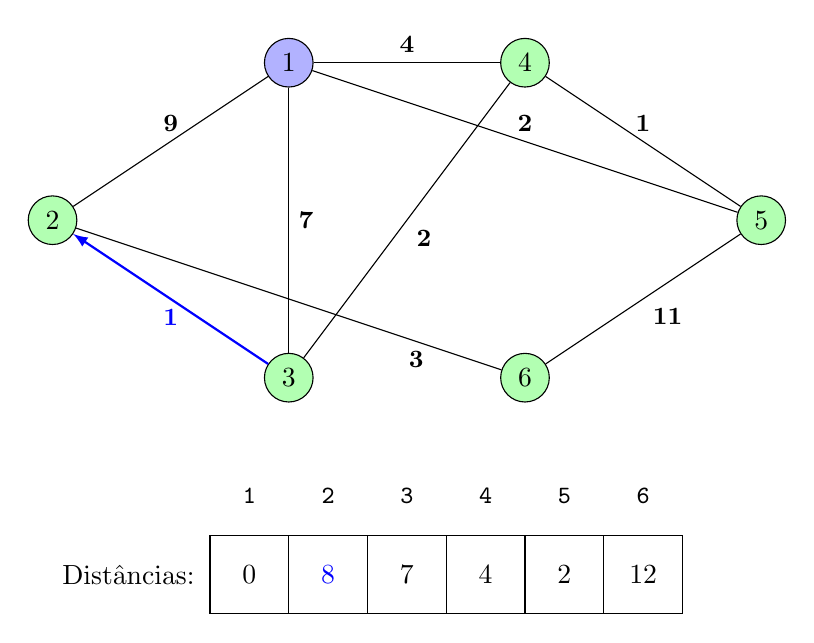
\begin{tikzpicture}
        \node[anchor=west] at (0, 0.5) { Distâncias: };

        \node[circle, draw, fill=blue!30] (a) at (3, 7) {1};
        \node[circle, draw, fill=green!30] (b) at (0, 5) {2};
        \node[circle, draw, fill=green!30] (c) at (3, 3) {3};
        \node[circle, draw, fill=green!30] (d) at (6, 7) {4};
        \node[circle, draw, fill=green!30] (e) at (9, 5) {5};
        \node[circle, draw, fill=green!30] (f) at (6, 3) {6};

        \draw (2, 0) grid (8, 1);

        \node at (2.5, 0.5) { $0$ };
        \node at (3.5, 0.5) { \textcolor{blue}{$8$} };
        \node at (4.5, 0.5) { \textcolor{black}{$7$} };
        \node at (5.5, 0.5) { \textcolor{black}{$4$} };
        \node at (6.5, 0.5) { \textcolor{black}{$2$} };
        \node at (7.5, 0.5) { \textcolor{black}{$12$} };

        \node at (2.5, 1.5) { \small \texttt{1} };
        \node at (3.5, 1.5) { \small \texttt{2} };
        \node at (4.5, 1.5) { \small \texttt{3} };
        \node at (5.5, 1.5) { \small \texttt{4} };
        \node at (6.5, 1.5) { \small \texttt{5} };
        \node at (7.5, 1.5) { \small \texttt{6} };

        \draw (a) to node[midway,anchor=south] { \small \bfseries 9 } (b);
        \draw (a) to node[midway,anchor=west] { \small \bfseries 7 } (c);
        \draw (a) to node[midway,anchor=south] { \small \bfseries 4 } (d);
        \draw (a) to node[midway,anchor=south] { \small \bfseries 2 } (e);
        %\draw (b) to node[midway,anchor=north] { \small \bfseries 1 } (c);
        \draw[latex-,thick,blue] (b) to node[midway,anchor=north] { \small \bfseries 1 } (c);
        \draw (b) to node[pos=0.8,anchor=north] { \small \bfseries 3 } (f);
        \draw (c) to node[midway,anchor=north west] { \small \bfseries 2 } (d);
        \draw (d) to node[midway,anchor=south] { \small \bfseries 1 } (e);
        \draw (e) to node[midway,anchor=north west] { \small \bfseries 11 } (f);

    \end{tikzpicture}

\end{frame}

\begin{frame}[fragile]{Visualização do algoritmo de Bellman-Ford}

    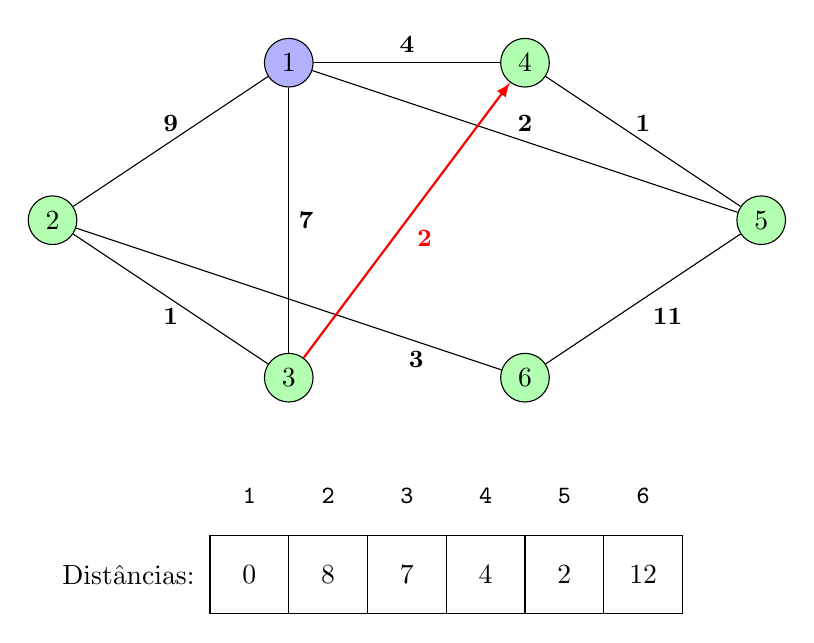
\begin{tikzpicture}
        \node[anchor=west] at (0, 0.5) { Distâncias: };

        \node[circle, draw, fill=blue!30] (a) at (3, 7) {1};
        \node[circle, draw, fill=green!30] (b) at (0, 5) {2};
        \node[circle, draw, fill=green!30] (c) at (3, 3) {3};
        \node[circle, draw, fill=green!30] (d) at (6, 7) {4};
        \node[circle, draw, fill=green!30] (e) at (9, 5) {5};
        \node[circle, draw, fill=green!30] (f) at (6, 3) {6};

        \draw (2, 0) grid (8, 1);

        \node at (2.5, 0.5) { $0$ };
        \node at (3.5, 0.5) { \textcolor{black}{$8$} };
        \node at (4.5, 0.5) { \textcolor{black}{$7$} };
        \node at (5.5, 0.5) { \textcolor{black}{$4$} };
        \node at (6.5, 0.5) { \textcolor{black}{$2$} };
        \node at (7.5, 0.5) { \textcolor{black}{$12$} };

        \node at (2.5, 1.5) { \small \texttt{1} };
        \node at (3.5, 1.5) { \small \texttt{2} };
        \node at (4.5, 1.5) { \small \texttt{3} };
        \node at (5.5, 1.5) { \small \texttt{4} };
        \node at (6.5, 1.5) { \small \texttt{5} };
        \node at (7.5, 1.5) { \small \texttt{6} };

        \draw (a) to node[midway,anchor=south] { \small \bfseries 9 } (b);
        \draw (a) to node[midway,anchor=west] { \small \bfseries 7 } (c);
        \draw (a) to node[midway,anchor=south] { \small \bfseries 4 } (d);
        \draw (a) to node[midway,anchor=south] { \small \bfseries 2 } (e);
        \draw (b) to node[midway,anchor=north] { \small \bfseries 1 } (c);
        \draw (b) to node[pos=0.8,anchor=north] { \small \bfseries 3 } (f);
        %\draw (c) to node[midway,anchor=north west] { \small \bfseries 2 } (d);
        \draw[-latex,thick,red] (c) to node[midway,anchor=north west] { \small \bfseries 2 } (d);
        \draw (d) to node[midway,anchor=south] { \small \bfseries 1 } (e);
        \draw (e) to node[midway,anchor=north west] { \small \bfseries 11 } (f);

    \end{tikzpicture}

\end{frame}

\begin{frame}[fragile]{Visualização do algoritmo de Bellman-Ford}

    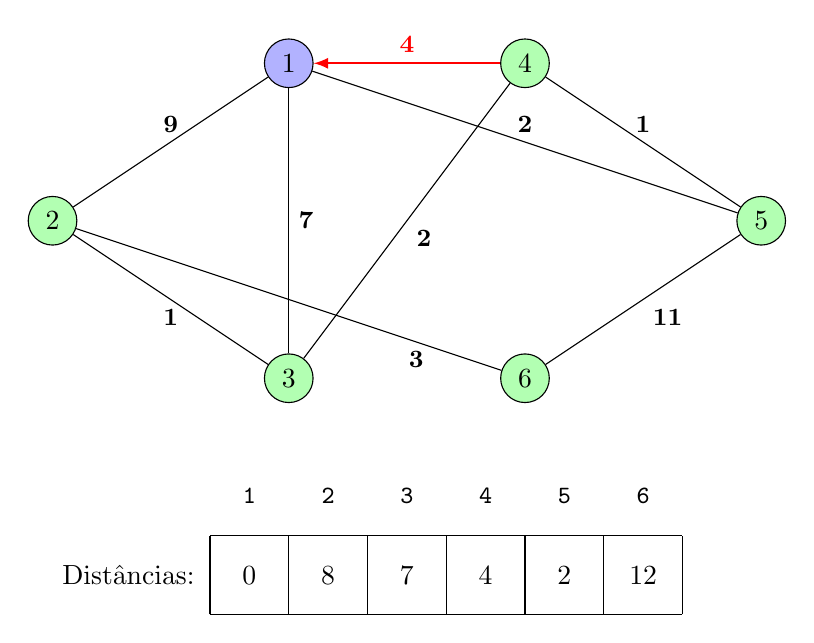
\begin{tikzpicture}
        \node[anchor=west] at (0, 0.5) { Distâncias: };

        \node[circle, draw, fill=blue!30] (a) at (3, 7) {1};
        \node[circle, draw, fill=green!30] (b) at (0, 5) {2};
        \node[circle, draw, fill=green!30] (c) at (3, 3) {3};
        \node[circle, draw, fill=green!30] (d) at (6, 7) {4};
        \node[circle, draw, fill=green!30] (e) at (9, 5) {5};
        \node[circle, draw, fill=green!30] (f) at (6, 3) {6};

        \draw (2, 0) grid (8, 1);

        \node at (2.5, 0.5) { $0$ };
        \node at (3.5, 0.5) { \textcolor{black}{$8$} };
        \node at (4.5, 0.5) { \textcolor{black}{$7$} };
        \node at (5.5, 0.5) { \textcolor{black}{$4$} };
        \node at (6.5, 0.5) { \textcolor{black}{$2$} };
        \node at (7.5, 0.5) { \textcolor{black}{$12$} };

        \node at (2.5, 1.5) { \small \texttt{1} };
        \node at (3.5, 1.5) { \small \texttt{2} };
        \node at (4.5, 1.5) { \small \texttt{3} };
        \node at (5.5, 1.5) { \small \texttt{4} };
        \node at (6.5, 1.5) { \small \texttt{5} };
        \node at (7.5, 1.5) { \small \texttt{6} };

        \draw (a) to node[midway,anchor=south] { \small \bfseries 9 } (b);
        \draw (a) to node[midway,anchor=west] { \small \bfseries 7 } (c);
        %\draw (a) to node[midway,anchor=south] { \small \bfseries 4 } (d);
        \draw[latex-,thick,red] (a) to node[midway,anchor=south] { \small \bfseries 4 } (d);
        \draw (a) to node[midway,anchor=south] { \small \bfseries 2 } (e);
        \draw (b) to node[midway,anchor=north] { \small \bfseries 1 } (c);
        \draw (b) to node[pos=0.8,anchor=north] { \small \bfseries 3 } (f);
        \draw (c) to node[midway,anchor=north west] { \small \bfseries 2 } (d);
        \draw (d) to node[midway,anchor=south] { \small \bfseries 1 } (e);
        \draw (e) to node[midway,anchor=north west] { \small \bfseries 11 } (f);

    \end{tikzpicture}

\end{frame}

\begin{frame}[fragile]{Visualização do algoritmo de Bellman-Ford}

    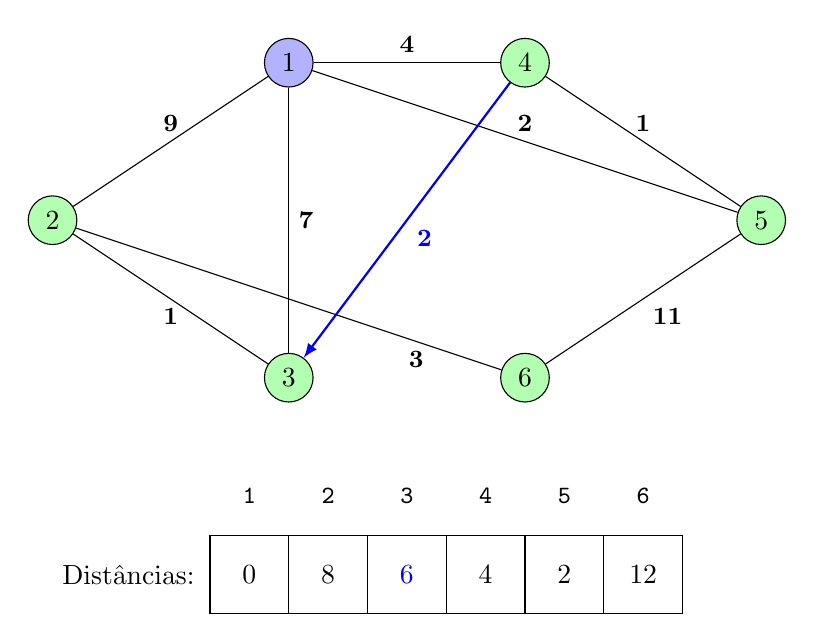
\begin{tikzpicture}
        \node[anchor=west] at (0, 0.5) { Distâncias: };

        \node[circle, draw, fill=blue!30] (a) at (3, 7) {1};
        \node[circle, draw, fill=green!30] (b) at (0, 5) {2};
        \node[circle, draw, fill=green!30] (c) at (3, 3) {3};
        \node[circle, draw, fill=green!30] (d) at (6, 7) {4};
        \node[circle, draw, fill=green!30] (e) at (9, 5) {5};
        \node[circle, draw, fill=green!30] (f) at (6, 3) {6};

        \draw (2, 0) grid (8, 1);

        \node at (2.5, 0.5) { $0$ };
        \node at (3.5, 0.5) { \textcolor{black}{$8$} };
        \node at (4.5, 0.5) { \textcolor{blue}{$6$} };
        \node at (5.5, 0.5) { \textcolor{black}{$4$} };
        \node at (6.5, 0.5) { \textcolor{black}{$2$} };
        \node at (7.5, 0.5) { \textcolor{black}{$12$} };

        \node at (2.5, 1.5) { \small \texttt{1} };
        \node at (3.5, 1.5) { \small \texttt{2} };
        \node at (4.5, 1.5) { \small \texttt{3} };
        \node at (5.5, 1.5) { \small \texttt{4} };
        \node at (6.5, 1.5) { \small \texttt{5} };
        \node at (7.5, 1.5) { \small \texttt{6} };

        \draw (a) to node[midway,anchor=south] { \small \bfseries 9 } (b);
        \draw (a) to node[midway,anchor=west] { \small \bfseries 7 } (c);
        \draw (a) to node[midway,anchor=south] { \small \bfseries 4 } (d);
        \draw (a) to node[midway,anchor=south] { \small \bfseries 2 } (e);
        \draw (b) to node[midway,anchor=north] { \small \bfseries 1 } (c);
        \draw (b) to node[pos=0.8,anchor=north] { \small \bfseries 3 } (f);
        \draw[latex-,thick,blue] (c) to node[midway,anchor=north west] { \small \bfseries 2 } (d);
        \draw (d) to node[midway,anchor=south] { \small \bfseries 1 } (e);
        \draw (e) to node[midway,anchor=north west] { \small \bfseries 11 } (f);

    \end{tikzpicture}

\end{frame}



\begin{frame}[fragile]{Visualização do algoritmo de Bellman-Ford}

    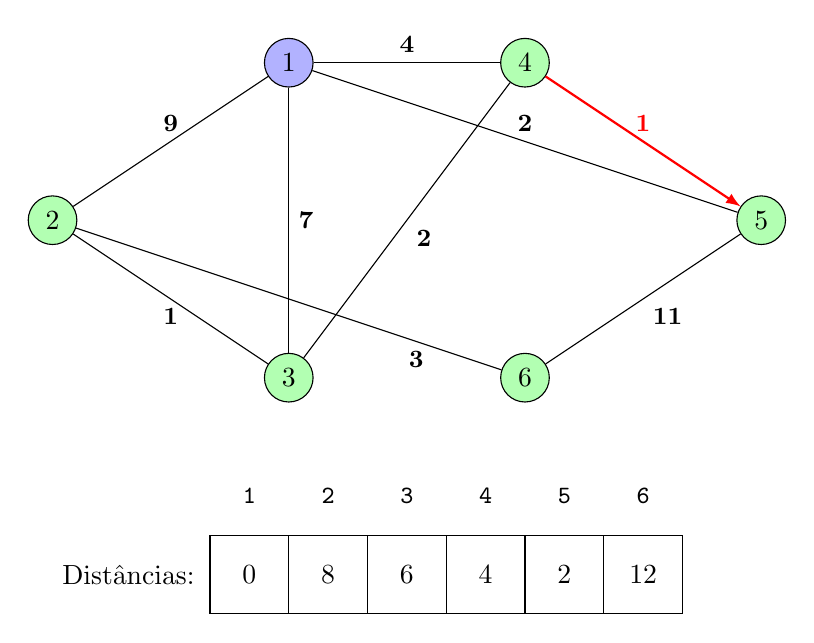
\begin{tikzpicture}
        \node[anchor=west] at (0, 0.5) { Distâncias: };

        \node[circle, draw, fill=blue!30] (a) at (3, 7) {1};
        \node[circle, draw, fill=green!30] (b) at (0, 5) {2};
        \node[circle, draw, fill=green!30] (c) at (3, 3) {3};
        \node[circle, draw, fill=green!30] (d) at (6, 7) {4};
        \node[circle, draw, fill=green!30] (e) at (9, 5) {5};
        \node[circle, draw, fill=green!30] (f) at (6, 3) {6};

        \draw (2, 0) grid (8, 1);

        \node at (2.5, 0.5) { $0$ };
        \node at (3.5, 0.5) { \textcolor{black}{$8$} };
        \node at (4.5, 0.5) { \textcolor{black}{$6$} };
        \node at (5.5, 0.5) { \textcolor{black}{$4$} };
        \node at (6.5, 0.5) { \textcolor{black}{$2$} };
        \node at (7.5, 0.5) { \textcolor{black}{$12$} };

        \node at (2.5, 1.5) { \small \texttt{1} };
        \node at (3.5, 1.5) { \small \texttt{2} };
        \node at (4.5, 1.5) { \small \texttt{3} };
        \node at (5.5, 1.5) { \small \texttt{4} };
        \node at (6.5, 1.5) { \small \texttt{5} };
        \node at (7.5, 1.5) { \small \texttt{6} };

        \draw (a) to node[midway,anchor=south] { \small \bfseries 9 } (b);
        \draw (a) to node[midway,anchor=west] { \small \bfseries 7 } (c);
        \draw (a) to node[midway,anchor=south] { \small \bfseries 4 } (d);
        \draw (a) to node[midway,anchor=south] { \small \bfseries 2 } (e);
        \draw (b) to node[midway,anchor=north] { \small \bfseries 1 } (c);
        \draw (b) to node[pos=0.8,anchor=north] { \small \bfseries 3 } (f);
        \draw (c) to node[midway,anchor=north west] { \small \bfseries 2 } (d);
        %\draw (d) to node[midway,anchor=south] { \small \bfseries 1 } (e);
        \draw[-latex,thick,red] (d) to node[midway,anchor=south] { \small \bfseries 1 } (e);
        \draw (e) to node[midway,anchor=north west] { \small \bfseries 11 } (f);

    \end{tikzpicture}

\end{frame}

\begin{frame}[fragile]{Visualização do algoritmo de Bellman-Ford}

    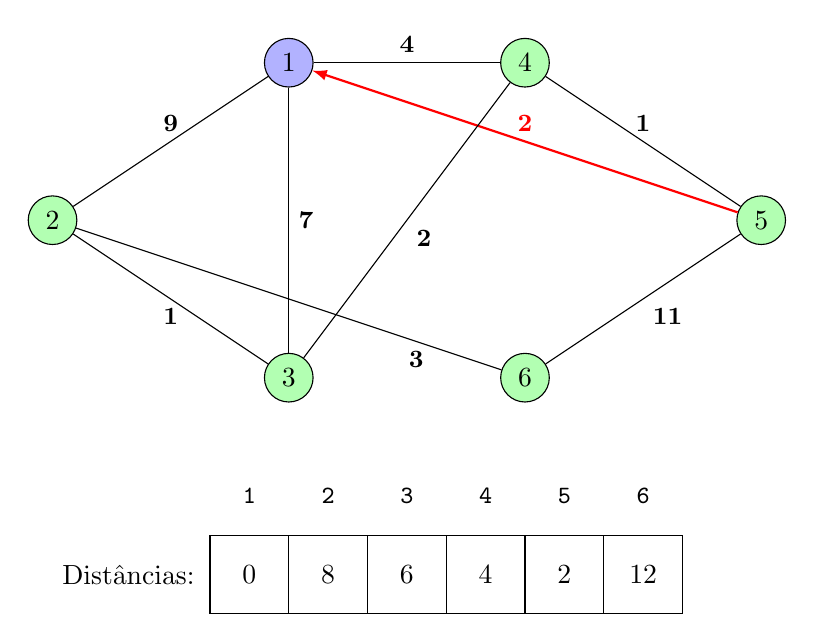
\begin{tikzpicture}
        \node[anchor=west] at (0, 0.5) { Distâncias: };

        \node[circle, draw, fill=blue!30] (a) at (3, 7) {1};
        \node[circle, draw, fill=green!30] (b) at (0, 5) {2};
        \node[circle, draw, fill=green!30] (c) at (3, 3) {3};
        \node[circle, draw, fill=green!30] (d) at (6, 7) {4};
        \node[circle, draw, fill=green!30] (e) at (9, 5) {5};
        \node[circle, draw, fill=green!30] (f) at (6, 3) {6};

        \draw (2, 0) grid (8, 1);

        \node at (2.5, 0.5) { $0$ };
        \node at (3.5, 0.5) { \textcolor{black}{$8$} };
        \node at (4.5, 0.5) { \textcolor{black}{$6$} };
        \node at (5.5, 0.5) { \textcolor{black}{$4$} };
        \node at (6.5, 0.5) { \textcolor{black}{$2$} };
        \node at (7.5, 0.5) { \textcolor{black}{$12$} };

        \node at (2.5, 1.5) { \small \texttt{1} };
        \node at (3.5, 1.5) { \small \texttt{2} };
        \node at (4.5, 1.5) { \small \texttt{3} };
        \node at (5.5, 1.5) { \small \texttt{4} };
        \node at (6.5, 1.5) { \small \texttt{5} };
        \node at (7.5, 1.5) { \small \texttt{6} };

        \draw (a) to node[midway,anchor=south] { \small \bfseries 9 } (b);
        \draw (a) to node[midway,anchor=west] { \small \bfseries 7 } (c);
        \draw (a) to node[midway,anchor=south] { \small \bfseries 4 } (d);
        %\draw (a) to node[midway,anchor=south] { \small \bfseries 2 } (e);
        \draw[latex-,thick,red] (a) to node[midway,anchor=south] { \small \bfseries 2 } (e);
        \draw (b) to node[midway,anchor=north] { \small \bfseries 1 } (c);
        \draw (b) to node[pos=0.8,anchor=north] { \small \bfseries 3 } (f);
        \draw (c) to node[midway,anchor=north west] { \small \bfseries 2 } (d);
        \draw (d) to node[midway,anchor=south] { \small \bfseries 1 } (e);
        \draw (e) to node[midway,anchor=north west] { \small \bfseries 11 } (f);

    \end{tikzpicture}

\end{frame}

\begin{frame}[fragile]{Visualização do algoritmo de Bellman-Ford}

    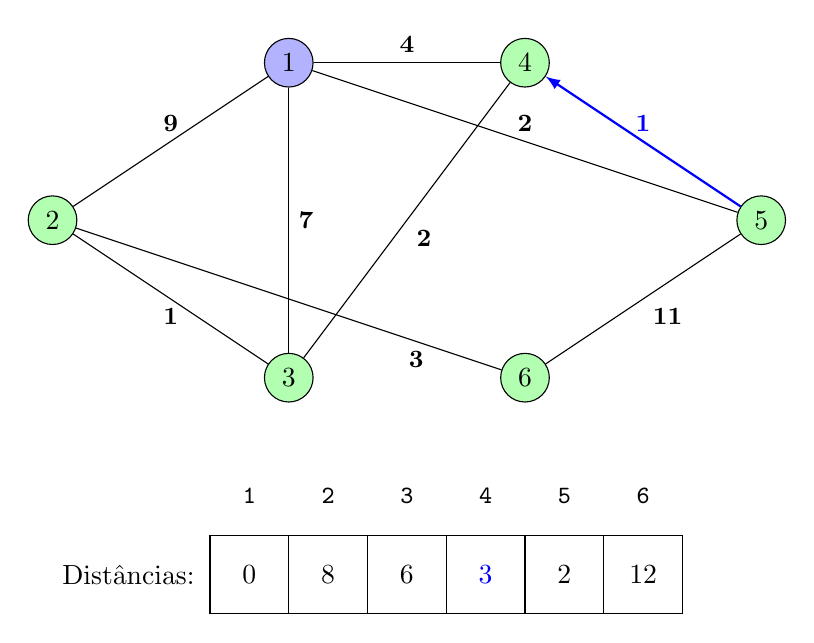
\begin{tikzpicture}
        \node[anchor=west] at (0, 0.5) { Distâncias: };

        \node[circle, draw, fill=blue!30] (a) at (3, 7) {1};
        \node[circle, draw, fill=green!30] (b) at (0, 5) {2};
        \node[circle, draw, fill=green!30] (c) at (3, 3) {3};
        \node[circle, draw, fill=green!30] (d) at (6, 7) {4};
        \node[circle, draw, fill=green!30] (e) at (9, 5) {5};
        \node[circle, draw, fill=green!30] (f) at (6, 3) {6};

        \draw (2, 0) grid (8, 1);

        \node at (2.5, 0.5) { $0$ };
        \node at (3.5, 0.5) { \textcolor{black}{$8$} };
        \node at (4.5, 0.5) { \textcolor{black}{$6$} };
        \node at (5.5, 0.5) { \textcolor{blue}{$3$} };
        \node at (6.5, 0.5) { \textcolor{black}{$2$} };
        \node at (7.5, 0.5) { \textcolor{black}{$12$} };

        \node at (2.5, 1.5) { \small \texttt{1} };
        \node at (3.5, 1.5) { \small \texttt{2} };
        \node at (4.5, 1.5) { \small \texttt{3} };
        \node at (5.5, 1.5) { \small \texttt{4} };
        \node at (6.5, 1.5) { \small \texttt{5} };
        \node at (7.5, 1.5) { \small \texttt{6} };

        \draw (a) to node[midway,anchor=south] { \small \bfseries 9 } (b);
        \draw (a) to node[midway,anchor=west] { \small \bfseries 7 } (c);
        \draw (a) to node[midway,anchor=south] { \small \bfseries 4 } (d);
        \draw (a) to node[midway,anchor=south] { \small \bfseries 2 } (e);
        \draw (b) to node[midway,anchor=north] { \small \bfseries 1 } (c);
        \draw (b) to node[pos=0.8,anchor=north] { \small \bfseries 3 } (f);
        \draw (c) to node[midway,anchor=north west] { \small \bfseries 2 } (d);
        %\draw (d) to node[midway,anchor=south] { \small \bfseries 1 } (e);
        \draw[latex-,thick,blue] (d) to node[midway,anchor=south] { \small \bfseries 1 } (e);
        \draw (e) to node[midway,anchor=north west] { \small \bfseries 11 } (f);

    \end{tikzpicture}

\end{frame}

\begin{frame}[fragile]{Visualização do algoritmo de Bellman-Ford}

    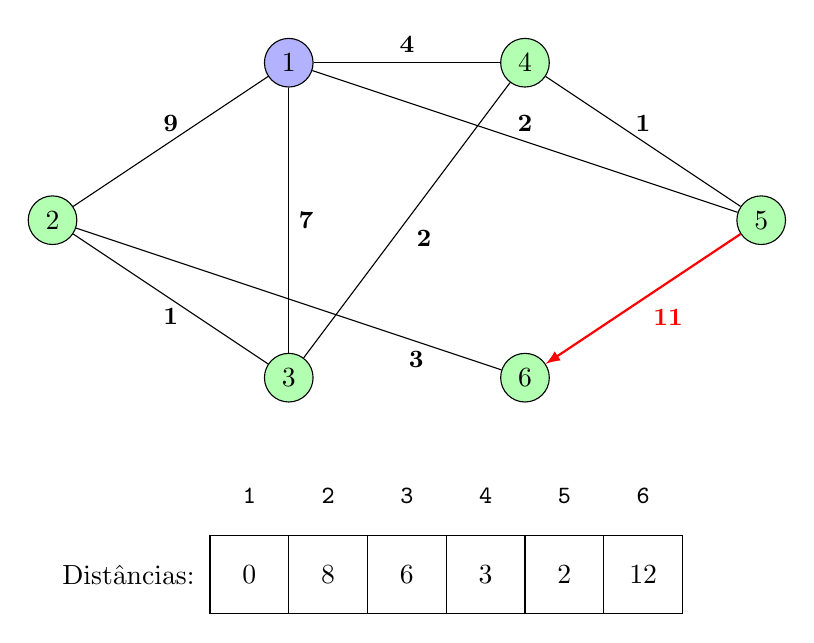
\begin{tikzpicture}
        \node[anchor=west] at (0, 0.5) { Distâncias: };

        \node[circle, draw, fill=blue!30] (a) at (3, 7) {1};
        \node[circle, draw, fill=green!30] (b) at (0, 5) {2};
        \node[circle, draw, fill=green!30] (c) at (3, 3) {3};
        \node[circle, draw, fill=green!30] (d) at (6, 7) {4};
        \node[circle, draw, fill=green!30] (e) at (9, 5) {5};
        \node[circle, draw, fill=green!30] (f) at (6, 3) {6};

        \draw (2, 0) grid (8, 1);

        \node at (2.5, 0.5) { $0$ };
        \node at (3.5, 0.5) { \textcolor{black}{$8$} };
        \node at (4.5, 0.5) { \textcolor{black}{$6$} };
        \node at (5.5, 0.5) { \textcolor{black}{$3$} };
        \node at (6.5, 0.5) { \textcolor{black}{$2$} };
        \node at (7.5, 0.5) { \textcolor{black}{$12$} };

        \node at (2.5, 1.5) { \small \texttt{1} };
        \node at (3.5, 1.5) { \small \texttt{2} };
        \node at (4.5, 1.5) { \small \texttt{3} };
        \node at (5.5, 1.5) { \small \texttt{4} };
        \node at (6.5, 1.5) { \small \texttt{5} };
        \node at (7.5, 1.5) { \small \texttt{6} };

        \draw (a) to node[midway,anchor=south] { \small \bfseries 9 } (b);
        \draw (a) to node[midway,anchor=west] { \small \bfseries 7 } (c);
        \draw (a) to node[midway,anchor=south] { \small \bfseries 4 } (d);
        \draw (a) to node[midway,anchor=south] { \small \bfseries 2 } (e);
        \draw (b) to node[midway,anchor=north] { \small \bfseries 1 } (c);
        \draw (b) to node[pos=0.8,anchor=north] { \small \bfseries 3 } (f);
        \draw (c) to node[midway,anchor=north west] { \small \bfseries 2 } (d);
        \draw (d) to node[midway,anchor=south] { \small \bfseries 1 } (e);
        %\draw (e) to node[midway,anchor=north west] { \small \bfseries 11 } (f);
        \draw[-latex,thick,red] (e) to node[midway,anchor=north west] { \small \bfseries 11 } (f);

    \end{tikzpicture}

\end{frame}


\begin{frame}[fragile]{Visualização do algoritmo de Bellman-Ford}

    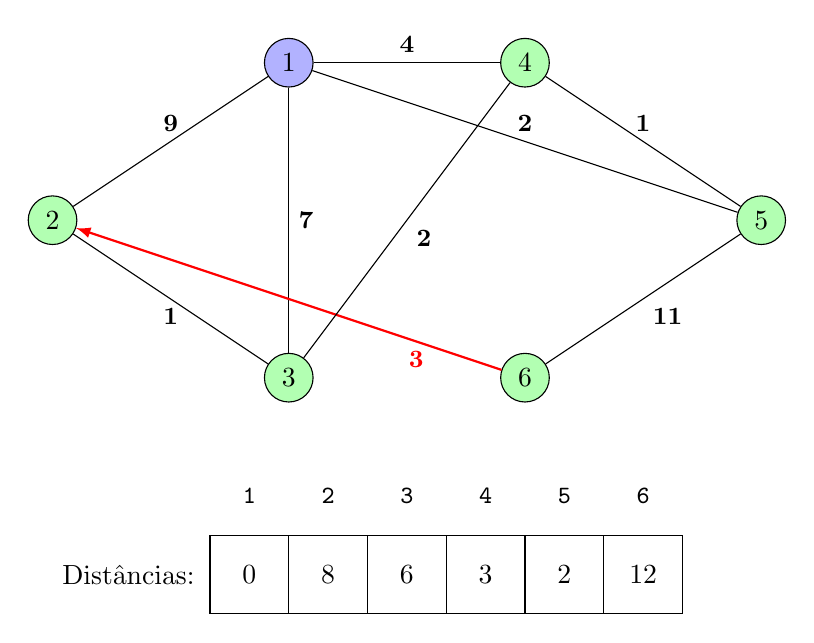
\begin{tikzpicture}
        \node[anchor=west] at (0, 0.5) { Distâncias: };

        \node[circle, draw, fill=blue!30] (a) at (3, 7) {1};
        \node[circle, draw, fill=green!30] (b) at (0, 5) {2};
        \node[circle, draw, fill=green!30] (c) at (3, 3) {3};
        \node[circle, draw, fill=green!30] (d) at (6, 7) {4};
        \node[circle, draw, fill=green!30] (e) at (9, 5) {5};
        \node[circle, draw, fill=green!30] (f) at (6, 3) {6};

        \draw (2, 0) grid (8, 1);

        \node at (2.5, 0.5) { $0$ };
        \node at (3.5, 0.5) { \textcolor{black}{$8$} };
        \node at (4.5, 0.5) { \textcolor{black}{$6$} };
        \node at (5.5, 0.5) { \textcolor{black}{$3$} };
        \node at (6.5, 0.5) { \textcolor{black}{$2$} };
        \node at (7.5, 0.5) { \textcolor{black}{$12$} };

        \node at (2.5, 1.5) { \small \texttt{1} };
        \node at (3.5, 1.5) { \small \texttt{2} };
        \node at (4.5, 1.5) { \small \texttt{3} };
        \node at (5.5, 1.5) { \small \texttt{4} };
        \node at (6.5, 1.5) { \small \texttt{5} };
        \node at (7.5, 1.5) { \small \texttt{6} };

        \draw (a) to node[midway,anchor=south] { \small \bfseries 9 } (b);
        \draw (a) to node[midway,anchor=west] { \small \bfseries 7 } (c);
        \draw (a) to node[midway,anchor=south] { \small \bfseries 4 } (d);
        \draw (a) to node[midway,anchor=south] { \small \bfseries 2 } (e);
        \draw (b) to node[midway,anchor=north] { \small \bfseries 1 } (c);
        %\draw (b) to node[pos=0.8,anchor=north] { \small \bfseries 3 } (f);
        \draw[latex-,thick,red] (b) to node[pos=0.8,anchor=north] { \small \bfseries 3 } (f);
        \draw (c) to node[midway,anchor=north west] { \small \bfseries 2 } (d);
        \draw (d) to node[midway,anchor=south] { \small \bfseries 1 } (e);
        \draw (e) to node[midway,anchor=north west] { \small \bfseries 11 } (f);

    \end{tikzpicture}

\end{frame}

\begin{frame}[fragile]{Visualização do algoritmo de Bellman-Ford}

    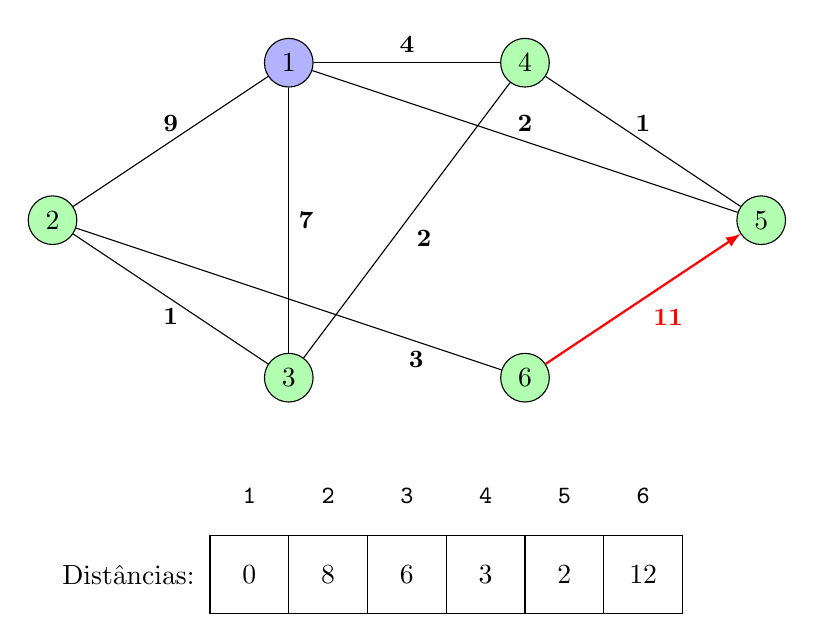
\begin{tikzpicture}
        \node[anchor=west] at (0, 0.5) { Distâncias: };

        \node[circle, draw, fill=blue!30] (a) at (3, 7) {1};
        \node[circle, draw, fill=green!30] (b) at (0, 5) {2};
        \node[circle, draw, fill=green!30] (c) at (3, 3) {3};
        \node[circle, draw, fill=green!30] (d) at (6, 7) {4};
        \node[circle, draw, fill=green!30] (e) at (9, 5) {5};
        \node[circle, draw, fill=green!30] (f) at (6, 3) {6};

        \draw (2, 0) grid (8, 1);

        \node at (2.5, 0.5) { $0$ };
        \node at (3.5, 0.5) { \textcolor{black}{$8$} };
        \node at (4.5, 0.5) { \textcolor{black}{$6$} };
        \node at (5.5, 0.5) { \textcolor{black}{$3$} };
        \node at (6.5, 0.5) { \textcolor{black}{$2$} };
        \node at (7.5, 0.5) { \textcolor{black}{$12$} };

        \node at (2.5, 1.5) { \small \texttt{1} };
        \node at (3.5, 1.5) { \small \texttt{2} };
        \node at (4.5, 1.5) { \small \texttt{3} };
        \node at (5.5, 1.5) { \small \texttt{4} };
        \node at (6.5, 1.5) { \small \texttt{5} };
        \node at (7.5, 1.5) { \small \texttt{6} };

        \draw (a) to node[midway,anchor=south] { \small \bfseries 9 } (b);
        \draw (a) to node[midway,anchor=west] { \small \bfseries 7 } (c);
        \draw (a) to node[midway,anchor=south] { \small \bfseries 4 } (d);
        \draw (a) to node[midway,anchor=south] { \small \bfseries 2 } (e);
        \draw (b) to node[midway,anchor=north] { \small \bfseries 1 } (c);
        \draw (b) to node[pos=0.8,anchor=north] { \small \bfseries 3 } (f);
        \draw (c) to node[midway,anchor=north west] { \small \bfseries 2 } (d);
        \draw (d) to node[midway,anchor=south] { \small \bfseries 1 } (e);
        %\draw (e) to node[midway,anchor=north west] { \small \bfseries 11 } (f);
        \draw[latex-,thick,red] (e) to node[midway,anchor=north west] { \small \bfseries 11 } (f);

    \end{tikzpicture}

\end{frame}

\begin{frame}[fragile]{Visualização do algoritmo de Bellman-Ford}

    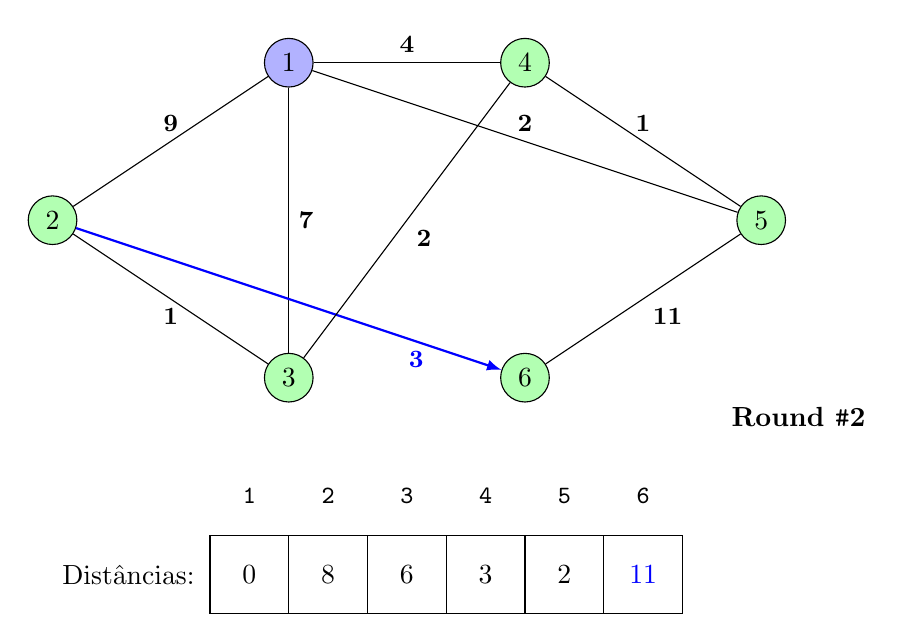
\begin{tikzpicture}
        \node[anchor=west] at (0, 0.5) { Distâncias: };
        \node[anchor=west] at (8.5, 2.5) { \bfseries Round \texttt{\#}2 };

        \node[circle, draw, fill=blue!30] (a) at (3, 7) {1};
        \node[circle, draw, fill=green!30] (b) at (0, 5) {2};
        \node[circle, draw, fill=green!30] (c) at (3, 3) {3};
        \node[circle, draw, fill=green!30] (d) at (6, 7) {4};
        \node[circle, draw, fill=green!30] (e) at (9, 5) {5};
        \node[circle, draw, fill=green!30] (f) at (6, 3) {6};

        \draw (2, 0) grid (8, 1);

        \node at (2.5, 0.5) { $0$ };
        \node at (3.5, 0.5) { \textcolor{black}{$8$} };
        \node at (4.5, 0.5) { \textcolor{black}{$6$} };
        \node at (5.5, 0.5) { \textcolor{black}{$3$} };
        \node at (6.5, 0.5) { \textcolor{black}{$2$} };
        \node at (7.5, 0.5) { \textcolor{blue}{$11$} };

        \node at (2.5, 1.5) { \small \texttt{1} };
        \node at (3.5, 1.5) { \small \texttt{2} };
        \node at (4.5, 1.5) { \small \texttt{3} };
        \node at (5.5, 1.5) { \small \texttt{4} };
        \node at (6.5, 1.5) { \small \texttt{5} };
        \node at (7.5, 1.5) { \small \texttt{6} };

        \draw (a) to node[midway,anchor=south] { \small \bfseries 9 } (b);
        \draw (a) to node[midway,anchor=west] { \small \bfseries 7 } (c);
        \draw (a) to node[midway,anchor=south] { \small \bfseries 4 } (d);
        \draw (a) to node[midway,anchor=south] { \small \bfseries 2 } (e);
        \draw (b) to node[midway,anchor=north] { \small \bfseries 1 } (c);
        \draw[-latex,thick,blue] (b) to node[pos=0.8,anchor=north] { \small \bfseries 3 } (f);
        \draw (c) to node[midway,anchor=north west] { \small \bfseries 2 } (d);
        \draw (d) to node[midway,anchor=south] { \small \bfseries 1 } (e);
        \draw (e) to node[midway,anchor=north west] { \small \bfseries 11 } (f);

    \end{tikzpicture}

\end{frame}

\begin{frame}[fragile]{Visualização do algoritmo de Bellman-Ford}

    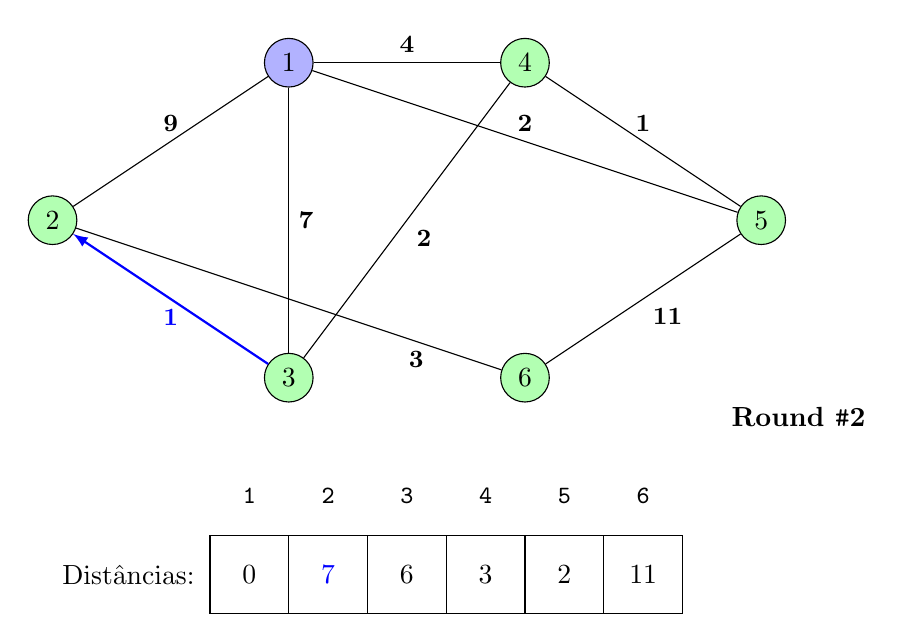
\begin{tikzpicture}
        \node[anchor=west] at (0, 0.5) { Distâncias: };
        \node[anchor=west] at (8.5, 2.5) { \bfseries Round \texttt{\#}2 };

        \node[circle, draw, fill=blue!30] (a) at (3, 7) {1};
        \node[circle, draw, fill=green!30] (b) at (0, 5) {2};
        \node[circle, draw, fill=green!30] (c) at (3, 3) {3};
        \node[circle, draw, fill=green!30] (d) at (6, 7) {4};
        \node[circle, draw, fill=green!30] (e) at (9, 5) {5};
        \node[circle, draw, fill=green!30] (f) at (6, 3) {6};

        \draw (2, 0) grid (8, 1);

        \node at (2.5, 0.5) { $0$ };
        \node at (3.5, 0.5) { \textcolor{blue}{$7$} };
        \node at (4.5, 0.5) { \textcolor{black}{$6$} };
        \node at (5.5, 0.5) { \textcolor{black}{$3$} };
        \node at (6.5, 0.5) { \textcolor{black}{$2$} };
        \node at (7.5, 0.5) { \textcolor{black}{$11$} };

        \node at (2.5, 1.5) { \small \texttt{1} };
        \node at (3.5, 1.5) { \small \texttt{2} };
        \node at (4.5, 1.5) { \small \texttt{3} };
        \node at (5.5, 1.5) { \small \texttt{4} };
        \node at (6.5, 1.5) { \small \texttt{5} };
        \node at (7.5, 1.5) { \small \texttt{6} };

        \draw (a) to node[midway,anchor=south] { \small \bfseries 9 } (b);
        \draw (a) to node[midway,anchor=west] { \small \bfseries 7 } (c);
        \draw (a) to node[midway,anchor=south] { \small \bfseries 4 } (d);
        \draw (a) to node[midway,anchor=south] { \small \bfseries 2 } (e);
        %\draw (b) to node[midway,anchor=north] { \small \bfseries 1 } (c);
        \draw[latex-,thick,blue](b) to node[midway,anchor=north] { \small \bfseries 1 } (c);
        \draw (b) to node[pos=0.8,anchor=north] { \small \bfseries 3 } (f);
        \draw (c) to node[midway,anchor=north west] { \small \bfseries 2 } (d);
        \draw (d) to node[midway,anchor=south] { \small \bfseries 1 } (e);
        \draw (e) to node[midway,anchor=north west] { \small \bfseries 11 } (f);

    \end{tikzpicture}

\end{frame}

\begin{frame}[fragile]{Visualização do algoritmo de Bellman-Ford}

    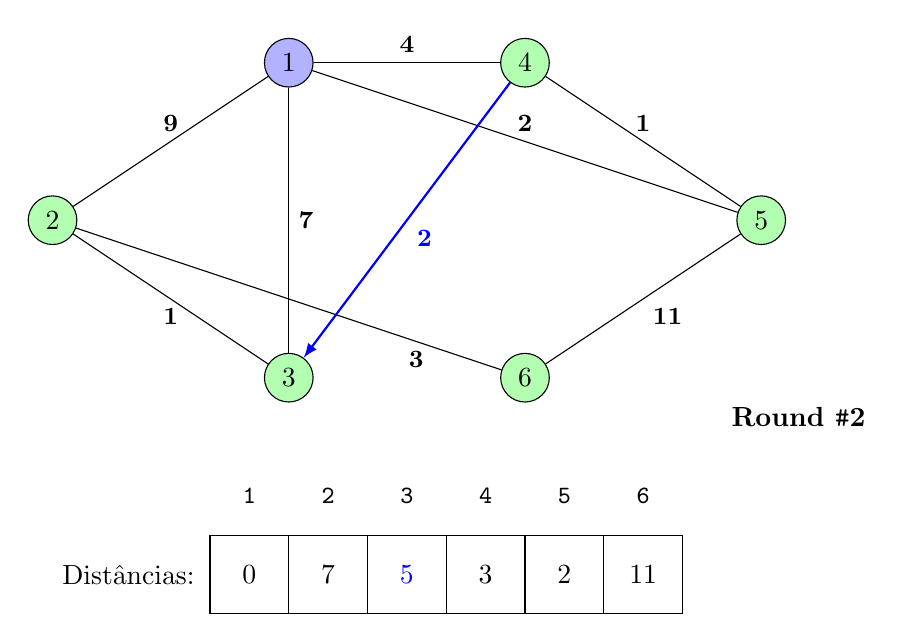
\begin{tikzpicture}
        \node[anchor=west] at (0, 0.5) { Distâncias: };
        \node[anchor=west] at (8.5, 2.5) { \bfseries Round \texttt{\#}2 };

        \node[circle, draw, fill=blue!30] (a) at (3, 7) {1};
        \node[circle, draw, fill=green!30] (b) at (0, 5) {2};
        \node[circle, draw, fill=green!30] (c) at (3, 3) {3};
        \node[circle, draw, fill=green!30] (d) at (6, 7) {4};
        \node[circle, draw, fill=green!30] (e) at (9, 5) {5};
        \node[circle, draw, fill=green!30] (f) at (6, 3) {6};

        \draw (2, 0) grid (8, 1);

        \node at (2.5, 0.5) { $0$ };
        \node at (3.5, 0.5) { \textcolor{black}{$7$} };
        \node at (4.5, 0.5) { \textcolor{blue}{$5$} };
        \node at (5.5, 0.5) { \textcolor{black}{$3$} };
        \node at (6.5, 0.5) { \textcolor{black}{$2$} };
        \node at (7.5, 0.5) { \textcolor{black}{$11$} };

        \node at (2.5, 1.5) { \small \texttt{1} };
        \node at (3.5, 1.5) { \small \texttt{2} };
        \node at (4.5, 1.5) { \small \texttt{3} };
        \node at (5.5, 1.5) { \small \texttt{4} };
        \node at (6.5, 1.5) { \small \texttt{5} };
        \node at (7.5, 1.5) { \small \texttt{6} };

        \draw (a) to node[midway,anchor=south] { \small \bfseries 9 } (b);
        \draw (a) to node[midway,anchor=west] { \small \bfseries 7 } (c);
        \draw (a) to node[midway,anchor=south] { \small \bfseries 4 } (d);
        \draw (a) to node[midway,anchor=south] { \small \bfseries 2 } (e);
        \draw (b) to node[midway,anchor=north] { \small \bfseries 1 } (c);
        \draw (b) to node[pos=0.8,anchor=north] { \small \bfseries 3 } (f);
        %\draw (c) to node[midway,anchor=north west] { \small \bfseries 2 } (d);
        \draw[latex-,thick,blue](c) to node[midway,anchor=north west] { \small \bfseries 2 } (d);
        \draw (d) to node[midway,anchor=south] { \small \bfseries 1 } (e);
        \draw (e) to node[midway,anchor=north west] { \small \bfseries 11 } (f);

    \end{tikzpicture}

\end{frame}

\begin{frame}[fragile]{Visualização do algoritmo de Bellman-Ford}

    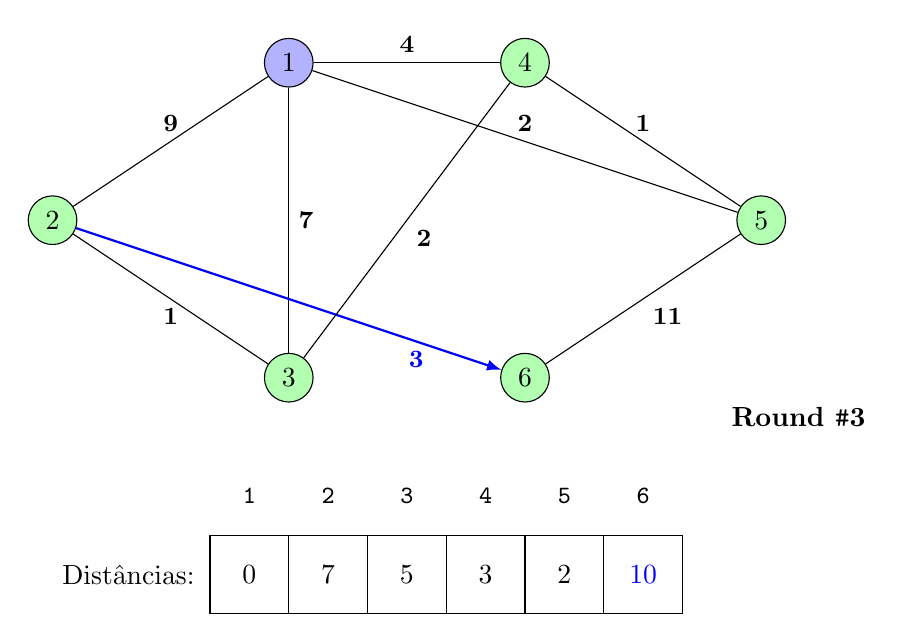
\begin{tikzpicture}
        \node[anchor=west] at (0, 0.5) { Distâncias: };
        \node[anchor=west] at (8.5, 2.5) { \bfseries Round \texttt{\#}3 };

        \node[circle, draw, fill=blue!30] (a) at (3, 7) {1};
        \node[circle, draw, fill=green!30] (b) at (0, 5) {2};
        \node[circle, draw, fill=green!30] (c) at (3, 3) {3};
        \node[circle, draw, fill=green!30] (d) at (6, 7) {4};
        \node[circle, draw, fill=green!30] (e) at (9, 5) {5};
        \node[circle, draw, fill=green!30] (f) at (6, 3) {6};

        \draw (2, 0) grid (8, 1);

        \node at (2.5, 0.5) { $0$ };
        \node at (3.5, 0.5) { \textcolor{black}{$7$} };
        \node at (4.5, 0.5) { \textcolor{black}{$5$} };
        \node at (5.5, 0.5) { \textcolor{black}{$3$} };
        \node at (6.5, 0.5) { \textcolor{black}{$2$} };
        \node at (7.5, 0.5) { \textcolor{blue}{$10$} };

        \node at (2.5, 1.5) { \small \texttt{1} };
        \node at (3.5, 1.5) { \small \texttt{2} };
        \node at (4.5, 1.5) { \small \texttt{3} };
        \node at (5.5, 1.5) { \small \texttt{4} };
        \node at (6.5, 1.5) { \small \texttt{5} };
        \node at (7.5, 1.5) { \small \texttt{6} };

        \draw (a) to node[midway,anchor=south] { \small \bfseries 9 } (b);
        \draw (a) to node[midway,anchor=west] { \small \bfseries 7 } (c);
        \draw (a) to node[midway,anchor=south] { \small \bfseries 4 } (d);
        \draw (a) to node[midway,anchor=south] { \small \bfseries 2 } (e);
        \draw (b) to node[midway,anchor=north] { \small \bfseries 1 } (c);
        %\draw (b) to node[pos=0.8,anchor=north] { \small \bfseries 3 } (f);
        \draw[-latex,thick,blue] (b) to node[pos=0.8,anchor=north] { \small \bfseries 3 } (f);
        \draw (c) to node[midway,anchor=north west] { \small \bfseries 2 } (d);
        \draw (d) to node[midway,anchor=south] { \small \bfseries 1 } (e);
        \draw (e) to node[midway,anchor=north west] { \small \bfseries 11 } (f);

    \end{tikzpicture}

\end{frame}

\begin{frame}[fragile]{Visualização do algoritmo de Bellman-Ford}

    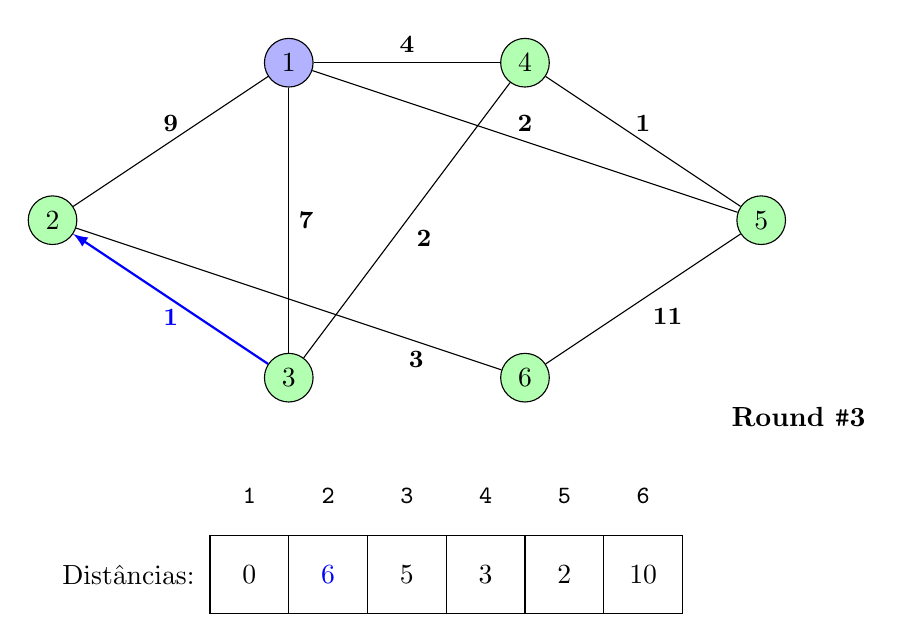
\begin{tikzpicture}
        \node[anchor=west] at (0, 0.5) { Distâncias: };
        \node[anchor=west] at (8.5, 2.5) { \bfseries Round \texttt{\#}3 };

        \node[circle, draw, fill=blue!30] (a) at (3, 7) {1};
        \node[circle, draw, fill=green!30] (b) at (0, 5) {2};
        \node[circle, draw, fill=green!30] (c) at (3, 3) {3};
        \node[circle, draw, fill=green!30] (d) at (6, 7) {4};
        \node[circle, draw, fill=green!30] (e) at (9, 5) {5};
        \node[circle, draw, fill=green!30] (f) at (6, 3) {6};

        \draw (2, 0) grid (8, 1);

        \node at (2.5, 0.5) { $0$ };
        \node at (3.5, 0.5) { \textcolor{blue}{$6$} };
        \node at (4.5, 0.5) { \textcolor{black}{$5$} };
        \node at (5.5, 0.5) { \textcolor{black}{$3$} };
        \node at (6.5, 0.5) { \textcolor{black}{$2$} };
        \node at (7.5, 0.5) { \textcolor{black}{$10$} };

        \node at (2.5, 1.5) { \small \texttt{1} };
        \node at (3.5, 1.5) { \small \texttt{2} };
        \node at (4.5, 1.5) { \small \texttt{3} };
        \node at (5.5, 1.5) { \small \texttt{4} };
        \node at (6.5, 1.5) { \small \texttt{5} };
        \node at (7.5, 1.5) { \small \texttt{6} };

        \draw (a) to node[midway,anchor=south] { \small \bfseries 9 } (b);
        \draw (a) to node[midway,anchor=west] { \small \bfseries 7 } (c);
        \draw (a) to node[midway,anchor=south] { \small \bfseries 4 } (d);
        \draw (a) to node[midway,anchor=south] { \small \bfseries 2 } (e);
        %\draw (b) to node[midway,anchor=north] { \small \bfseries 1 } (c);
        \draw[latex-,thick,blue] (b) to node[midway,anchor=north] { \small \bfseries 1 } (c);
        \draw (b) to node[pos=0.8,anchor=north] { \small \bfseries 3 } (f);
        \draw (c) to node[midway,anchor=north west] { \small \bfseries 2 } (d);
        \draw (d) to node[midway,anchor=south] { \small \bfseries 1 } (e);
        \draw (e) to node[midway,anchor=north west] { \small \bfseries 11 } (f);

    \end{tikzpicture}

\end{frame}

\begin{frame}[fragile]{Visualização do algoritmo de Bellman-Ford}

    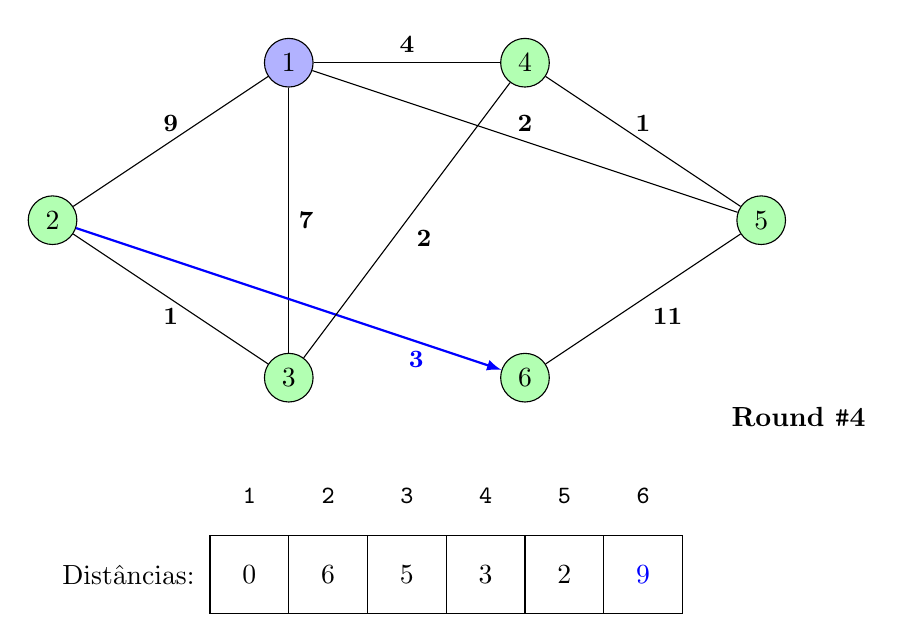
\begin{tikzpicture}
        \node[anchor=west] at (0, 0.5) { Distâncias: };
        \node[anchor=west] at (8.5, 2.5) { \bfseries Round \texttt{\#}4 };

        \node[circle, draw, fill=blue!30] (a) at (3, 7) {1};
        \node[circle, draw, fill=green!30] (b) at (0, 5) {2};
        \node[circle, draw, fill=green!30] (c) at (3, 3) {3};
        \node[circle, draw, fill=green!30] (d) at (6, 7) {4};
        \node[circle, draw, fill=green!30] (e) at (9, 5) {5};
        \node[circle, draw, fill=green!30] (f) at (6, 3) {6};

        \draw (2, 0) grid (8, 1);

        \node at (2.5, 0.5) { $0$ };
        \node at (3.5, 0.5) { \textcolor{black}{$6$} };
        \node at (4.5, 0.5) { \textcolor{black}{$5$} };
        \node at (5.5, 0.5) { \textcolor{black}{$3$} };
        \node at (6.5, 0.5) { \textcolor{black}{$2$} };
        \node at (7.5, 0.5) { \textcolor{blue}{$9$} };

        \node at (2.5, 1.5) { \small \texttt{1} };
        \node at (3.5, 1.5) { \small \texttt{2} };
        \node at (4.5, 1.5) { \small \texttt{3} };
        \node at (5.5, 1.5) { \small \texttt{4} };
        \node at (6.5, 1.5) { \small \texttt{5} };
        \node at (7.5, 1.5) { \small \texttt{6} };

        \draw (a) to node[midway,anchor=south] { \small \bfseries 9 } (b);
        \draw (a) to node[midway,anchor=west] { \small \bfseries 7 } (c);
        \draw (a) to node[midway,anchor=south] { \small \bfseries 4 } (d);
        \draw (a) to node[midway,anchor=south] { \small \bfseries 2 } (e);
        \draw (b) to node[midway,anchor=north] { \small \bfseries 1 } (c);
        %\draw (b) to node[pos=0.8,anchor=north] { \small \bfseries 3 } (f);
        \draw[-latex,thick,blue] (b) to node[pos=0.8,anchor=north] { \small \bfseries 3 } (f);
        \draw (c) to node[midway,anchor=north west] { \small \bfseries 2 } (d);
        \draw (d) to node[midway,anchor=south] { \small \bfseries 1 } (e);
        \draw (e) to node[midway,anchor=north west] { \small \bfseries 11 } (f);

    \end{tikzpicture}

\end{frame}
